%! Licence = CC BY-NC-SA 4.0

%! Author = gianfluetsch
%! Date = 19. Jan 2022
%! Project = pfsec_summary

\section{Access Control}

\subsection{Different types of access control}

\subsubsection{Controlling access to assets}
An access control is any hardware, software, or administrative policy or procedure that controls access to resources.

The goal is to provide access to authorized subjects and prevent unauthorized access attempts.\\
\begin{itemize}
    \item \textbf{Subject}
    \begin{itemize}
        \item A subject is an \textit{active entity that accesses a passive object} to receive information from, or data about, an object.
        \item Subjects can be users, programs, processes, services, computers, or anything else that can access a resource.
    \end{itemize}
    \item \textbf{Object}
    \begin{itemize}
        \item An object is a \textit{passive entity that provides information to active subjects}.
        \item Some examples of objects include files, databases, computers, programs, processes, services, printers, and storage media.\\
    \end{itemize}
\end{itemize}

The management of the relationship between subjects and objects is known as \textit{access control}.

\subsubsection{Primary Access Control Types}
\begin{itemize}
    \item \textbf{Preventive}
    \begin{itemize}
        \item A preventive control attempts to thwart or stop unwanted or unauthorized activity from occurring.
        \item \textit{Examples}: fences, locks, biometrics, mantraps, lighting, alarm systems, separation of duties, job rotation, data classification, penetration testing, encryption, auditing, security cameras, smartcards, security policies, securityawareness training, antivirus software, firewalls, intrusion prevention systems (IPS).
    \end{itemize}
    \item \textbf{Detective}
    \begin{itemize}
        \item  A detective control attempts to discover or detect unwanted or unauthorized activity.
        \item Detective controls operate after the fact and can discover the activity only after it has occurred.
        \item \textit{Examples}: security guards, motion detectors, recording and review of events captured by security cameras, job rotation, mandatory vacations, audit trails, honeypots, intrusion detection systems (IDSs), supervision and reviews of users, incident investigations.
    \end{itemize}
    \item \textbf{Corrective}
    \begin{itemize}
        \item A corrective control modifies the environment to return systems to normal after an unwanted or unauthorized activity has occurred. Corrective controls attempt to correct any problems that occurred because of a security incident.
        \item \textit{Examples}: Reboot of a system, antivirus solutions to remove or quarantine a virus, backup and restore plans to ensure that lost data can be restored.
    \end{itemize}
\end{itemize}

\subsubsection{Other Types of Access Control}
\begin{itemize}
    \item \textbf{Deterrent}
    \begin{itemize}
        \item A deterrent control is deployed to discourage violation of security policies. Deterrent and preventive controls are similar, but deterrent controls often depend on individuals deciding not to take an unwanted action. In contrast, a preventive control actually blocks the action.
        \item \textit{Examples}: Policies, security-awareness training, locks, fences, security badges, guards, mantraps, security cameras.        
    \end{itemize}
    \item \textbf{Compensating}
    \begin{itemize}
        \item A compensation control is deployed to provide various options to other existing controls to aid in enforcement and support of security policies. They can be any controls used in addition to, or in place of, another control.
        \item \textit{Examples}: An organizational policy dictating that all PII must be encrypted. If a preventive control is encrypting all PII data in databases but PII transferred over the network is sent in cleartext, a compensation control can be added to protect the data in transit.
    \end{itemize}
    \item \textbf{Recovery}
    \begin{itemize}
        \item Recovery controls are an extension of corrective controls but have more advanced or complex abilities.
        \item \textit{Examples}: Backups and restores, fault-tolerant drive systems, system imaging, server clustering, antivirus software, database or virtual machine shadowing, hot sites, warm sites, cold sites, alternate processing facilities, reciprocal agreements, cloud providers, rolling mobile operating centers, multisite solutions.
    \end{itemize}
    \item \textbf{Directive}
    \begin{itemize}
        \item A directive control is deployed to direct, confine, or control the actions of subjects to force or encourage compliance with security policies.
        \item Reine ''Papiermassnahme''
        \item \textit{Examples}: Security policy requirements or criteria, posted notifications, escape route exit signs, monitoring, supervision, procedures.
    \end{itemize}
\end{itemize}

\subsubsection{Implementation of Access Controls}\label{subsubsec:implementation-of-access-controls}
\begin{itemize}
    \item \textbf{Physical controls}
    \begin{itemize}
        \item Physikalische Präventivmassnahme, um z.B. nur einzelnen Personen Zutritt zum RZ gewähren
        \item items you can physically touch. Physical mechanisms deployed to prevent, monitor, or detect direct contact with systems or areas within a facility.
        \item \textit{Examples}: guards, fences, motion detectors, locked doors, sealed windows, lights, cable protection, laptop locks, badges, swipe cards, guard dogs, video cameras, mantraps, alarms
    \end{itemize}
    \item \textbf{Technical}
    \begin{itemize}
        \item It uses technology. It is the hardware or software mechanisms used to manage access and to provide protection for resources and systems.
        \item \textit{Examples}: authentication methods (such as usernames, passwords, smartcards, and biometrics), encryption, access control lists, protocols, firewalls, routers, intrusion detection systems (IDSs).
    \end{itemize}
    \item \textbf{Administrative}
    \begin{itemize}
        \item It focuses on personnel and business practices (Management controls). Policies and procedures defined by an organization's security policy.
        \item \textit{Examples}: policies, procedures, hiring practices, background checks, data classifications and labelling, security awareness and training efforts, vacation history, reports and reviews, work supervision, personnel controls and testing
    \end{itemize}
\end{itemize}

\begin{center}
    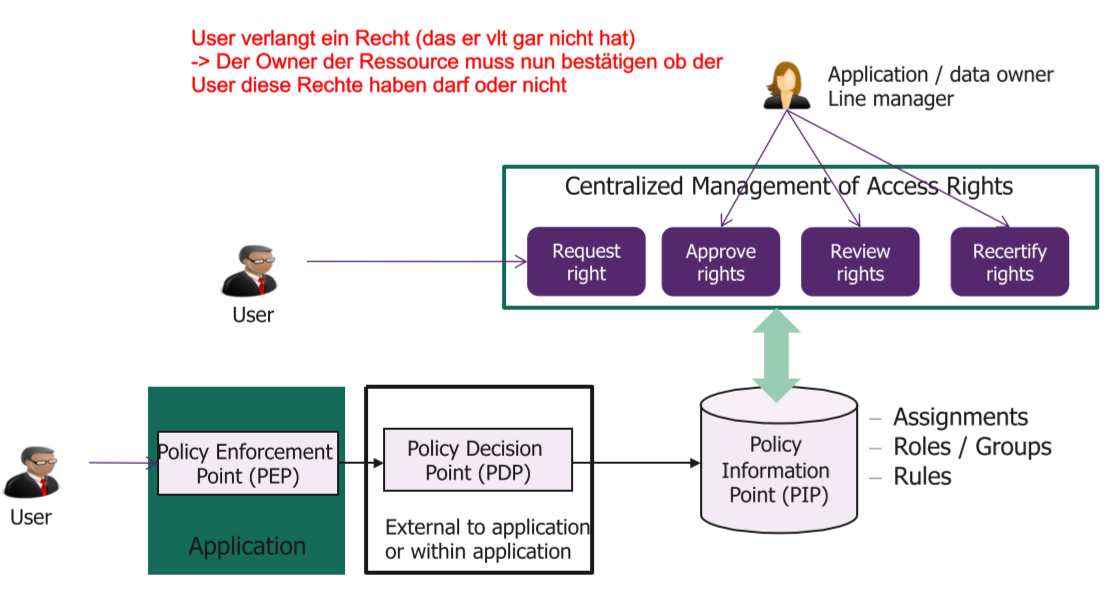
\includegraphics[width=.5\linewidth]{04-access_control/access_control}
    \vspace{-8pt}
\end{center}

\newpage

\subsubsection{Authorization Principles}
\begin{enumerate}
    \item \textbf{Implicit Deny}
    \begin{itemize}
        \item Basic principle of access control is implicit deny
        \item Most authorization mechanisms use it.
        \item The implicit deny principle ensures that access to an object (file) is denied unless access has been explicitly granted to a subject (user).
    \end{itemize}
    \item \textbf{Constrained Interface}
    \begin{itemize}
        \item Applications use constrained interfaces or restricted interfaces to restrict what users can do or see based on their privileges.
        \item Users with full privileges have access to all the capabilities of the application.
        \item A common method is to hide the capability if the user does not have permissions to use it.
    \end{itemize}
    \item \textbf{Content-Dependent Control}
    \begin{itemize}
        \item Restrict access to data based on the content within an object.
        \item Auf sensible/ persönliche Daten gibt es eine Access Control (oft bei Löhnen etc. so geregelt)
        \item A database view is a content-dependent control. A view retrieves specific columns from one or more tables, creating a virtual table.
    \end{itemize}
    \item \textbf{Context-Dependent Control}
    \begin{itemize}
        \item Context-dependent access controls require specific activity before granting users access.
        \item zur Run-Time (oft kein statisches Recht) $\rightarrow$ wird erst zur Laufzeit ausgewertet (Dynamisches Access Control)
        \item \textit{Example}: Data flow for a transaction selling digital products online. Users add products to a shopping cart, goes through the checkout process, enters credit card data. The last page confirms the purchase and provides instructions for downloading the digital products. The system denies access to the download page if users don't go through the purchase process first.
    \end{itemize}
    \item \textbf{Need to Know}
    \begin{itemize}
        \item This principle ensures that subjects are granted access only to what they need to know for their work tasks and job functions.
        \item auf Daten bezogen
        \item Subjects may have clearance to access classified or restricted data but are not granted authorization to the data unless they actually need it to perform a job.
    \end{itemize}
    \item \textbf{Least Privilege}
    \begin{itemize}
        \item The principle of least privilege ensures that subjects are granted only the privileges they need to perform their work tasks and job functions.
        \item Rechte auf System, mit Least Privilege werden mehr Ressourcen geschützt (nicht nur Daten wie bei ''Need to Know'')
        \item The principle of least privilege relies on the assumption that all users have a well-defined job description that personnel understand.
        \item Without a specific job description, it is not possible to know what privileges users need.
    \end{itemize}
    \item \textbf{Separation of Duties and Responsibilities}
    \begin{itemize}
        \item The principle ensures that no single person has total control over a critical function or system.
        \item \textcolor{red}{Im Access Control eines der wichtigsten Punkte}
    \end{itemize}
    \item \textbf{Transitive Trust}
    \begin{itemize}
        \item When A requests data from B and then B requests data from C, the data that A receives is essentially from C.
        \item \textcolor{red}{Transitive trust is a serious security concern because it may enable bypassing of restrictions or limitations between A and C.}
    \end{itemize}
    \item \textbf{Confinement}
    \begin{itemize}
        \item Process confinement allows a process to read from and write to only certain memory locations and resources.
        \item Confinement can be implemented in the OS itself, through the use of a confinement application or service or through a virtualization or hypervisor solution
    \end{itemize}
    \item \textbf{Isolation}
    \begin{itemize}
        \item When a process is confined through enforcing access bounds, that process runs in isolation.
        \item Isolation is an essential component of a stable operating system. Isolation is what prevents an application from accessing the memory or resources of another application.
    \end{itemize}
\end{enumerate}

\subsection{Security Models}

\subsubsection{Bell-LaPadula (Multi Level Security)}
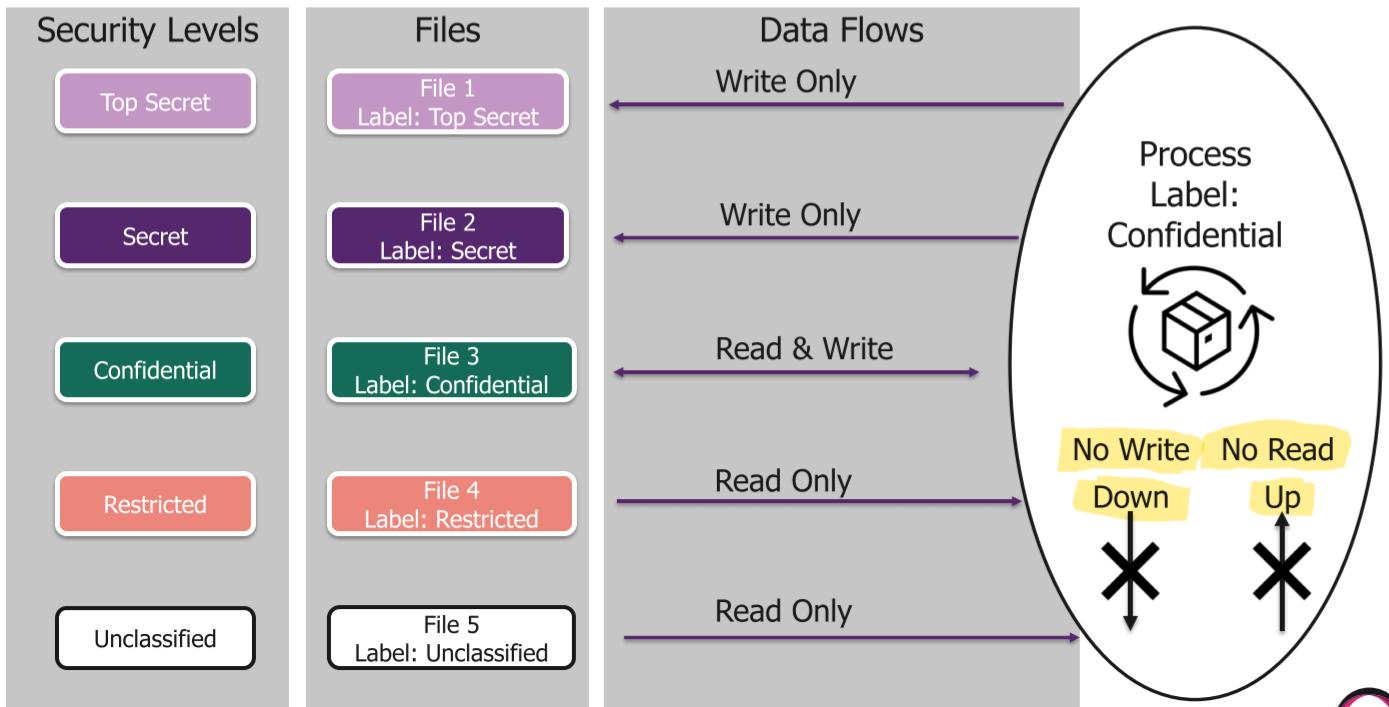
\includegraphics[width=.5\linewidth]{04-access_control/bell_lapadula}
\begin{itemize}
    \item Allows to create any number of \textit{Categories} or \textit{Compartments}
    \item Arose in the military out of the requirement of \textit{need to know}
    \item Restricts information flow between departments
\end{itemize}

\subsubsection{BIBA (Integrity)}
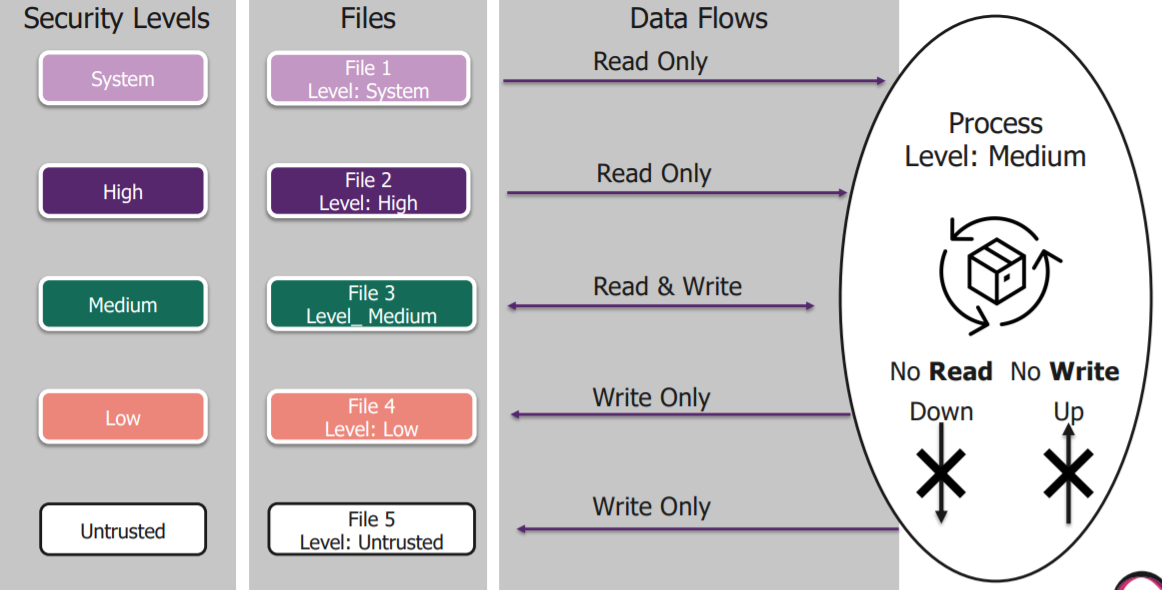
\includegraphics[width=.5\linewidth]{04-access_control/biba}

\subsubsection{Clark Wilson Model}
\begin{itemize}
    \item The Clark-Wilson model does not define a formal state machine and is not dependent on data classification.
    \begin{itemize}
        \item Subjects do not have direct access to objects.
        \item A subject is able to access objects only by using a program
        \item Objects can be accessed only through programs
        \item Well-formed transactions take the form of programs.
    \end{itemize}
    \item Each program has specific limitations on what it can and cannot do to an object (such as a database or other resource).
    \item The Clark-Wilson model enforces data integrity and separation of duties and that makes it a common model for commercial applications.
    \item Ähnlich wie Unix ACL System (rwx)
\end{itemize}

\subsubsection{Chinese Walls (Brewer Nash Model)}
\begin{itemize}
    \item Permit access controls to change dynamically based on a user's previous activity
    \item It seeks to create security domains that are sensitive to the notion of conflict of interest
    \begin{itemize}
        \item It creates conflict classes that defines which security domains are potentially in conflict
        \item It prevents any subject with access to one domain that belongs to a specific conflict class from accessing any other domain that belongs to the same conflict class.
    \end{itemize}
    \item It uses the principle of data isolation and supports separation of duties.
    \item Principle of Chinese Walls werden oft bei Admins Accounts in einer Firma angewendet
    -\begin{itemize}
        \item entweder als Admin oder als normaler User arbeiten
        \item aber nicht beides gleichzeitig (immer mit User mit Adminrechten arbeiten ist sehr schlecht!!!)
    \end{itemize}
\end{itemize}

\subsection{Access Control Models}
\begin{itemize}
    \item \textbf{Mandatory Access Control (MAC)}
    \begin{itemize}
        \item Controls access based on comparing security labels with security clearances.\\
    \end{itemize}
    \item \textbf{Discretionary Access Control (DAC)}
    \begin{itemize}
        \item Controls access based on the identity of the requestor and on access rules (authorizations) stating what requestors are (or are not) allowed to do.\\
    \end{itemize}
    \item \textbf{Role Based Access Control (RBAC)}
    \begin{itemize}
        \item Controls access based on the roles that users have within the system and on rules stating what accesses are allowed to users in given roles.\\
    \end{itemize}
    \item \textbf{Attribute Based Access Control (ABAC)}
    \begin{itemize}
        \item Controls access based on attributes of the user, the resource to be accessed, and current environmental conditions.
    \end{itemize}
\end{itemize}

\subsubsection{Discretionary Access Control (DAC)}
\begin{itemize}
    \item Access control policy is determined by the owner of an object.
    \item Every object has an owner.
    \item The owner can grant or deny access to any other subjects. It decides who is allowed to access the object and can define the privileges other users have with the object.
    \item NTFS uses the DAC model
    \item It is often provided using an access matrix:
    \begin{itemize}
        \item One dimension consists of identified subjects that may attempt data access to the resources
        \item The other dimension lists the objects that may be accessed
        \item Each entry in the matrix indicates the access rights of a particular subject for a particular object
    \end{itemize}
\end{itemize}

\begin{center}
    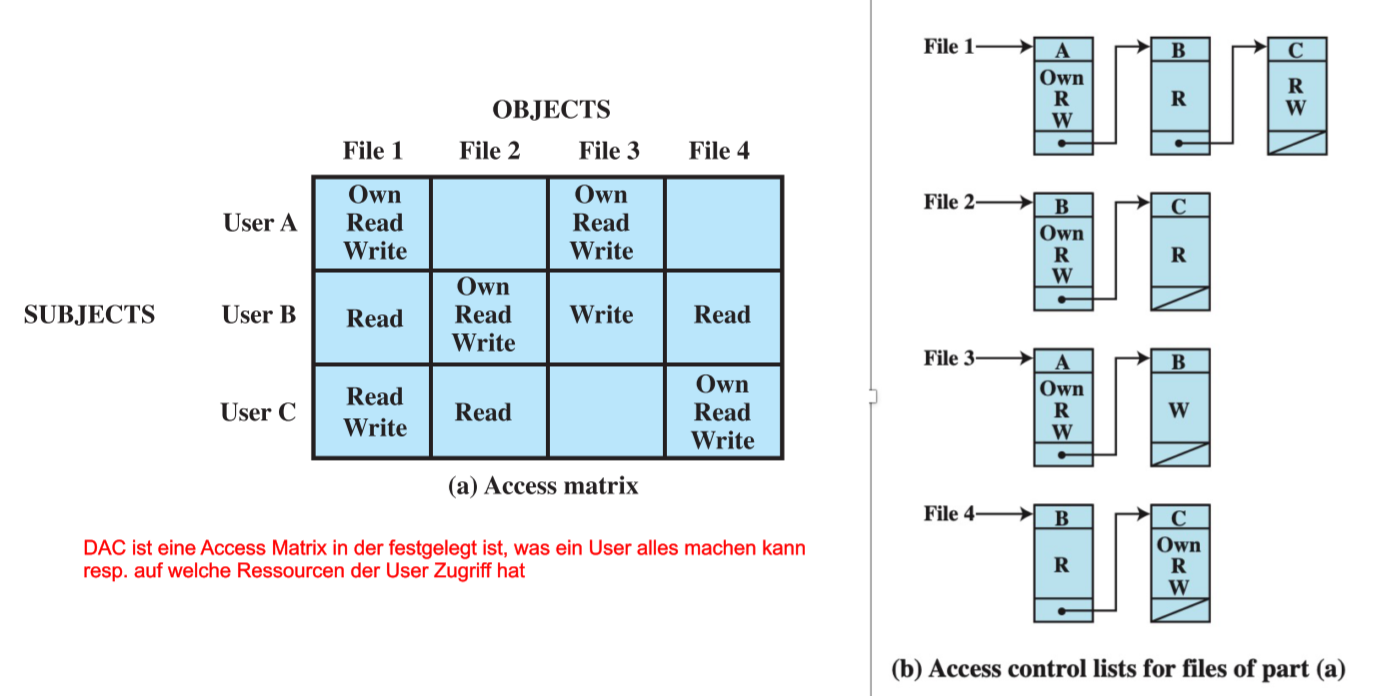
\includegraphics[width=0.9\linewidth]{04-access_control/dac}
    \vspace{-8pt}
\end{center}

\paragraph{Protection Domains}
\begin{itemize}
    \item Are a \textit{set of objects together with access rights to those objects}
    \item More flexibility when associating capabilities with protection domains
    \item \textbf{In terms of the access matrix, a row defines a protection domain}
    \item User can spawn processes with a subset of the access rights of the user
    \item Association between a process and a domain can be \textit{static} or \textit{dynamic}
    \item In user mode certain areas of memory are protected from use and certain instructions may not be executed
    \item In kernel mode privileged instructions may be executed and protected areas of memory may be accessed
\end{itemize}

\subsubsection{Role Based Access Control (RBAC)}
\begin{itemize}
    \item Access control policy is defined by the role[s] a user has
    \item Permissions are not assigned directly to users
    \item User accounts are placed in roles and administrators assign privileges to the roles. These roles are typically identified by job functions.
    \item If a user account is in a role, the user has all the privileges assigned to the role.\\
\end{itemize}

Permissions werden über Rollen verwaltet (Permission wird einer Rolle zugewiesen $\rightarrow$ wie in Active Directory mit ug, dlg, etc.)
Einem User wird nun die entsprechende Rolle (in AD eine ug) zugewiesen und über diese Rolle hat der User dann die entsprechende Berechtigung für eine Ressource, etc.

\begin{center}
    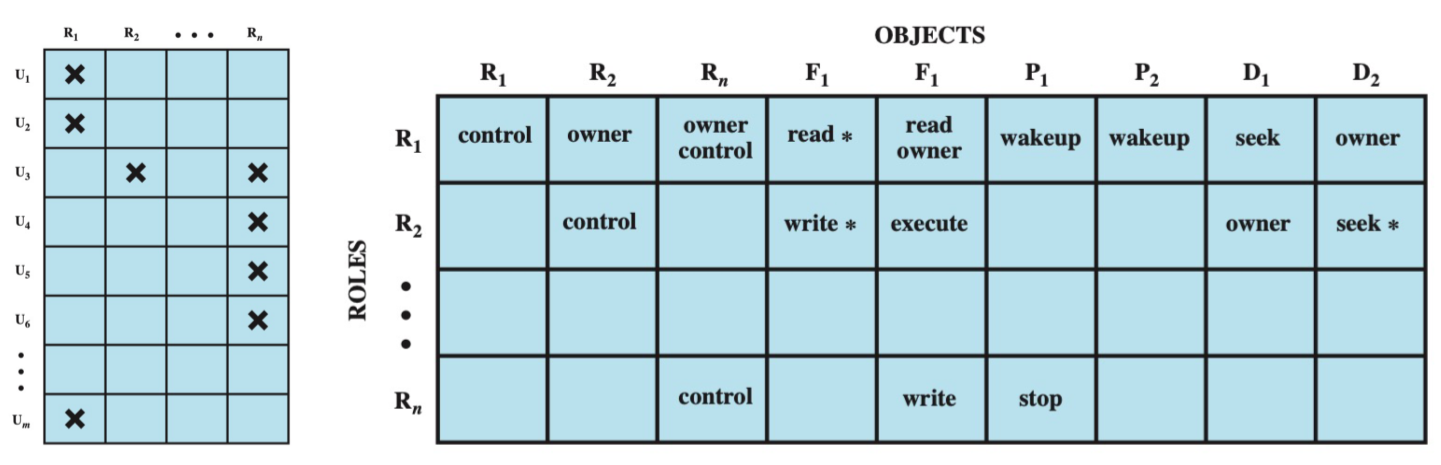
\includegraphics[width=1.0\linewidth]{04-access_control/rbac}
    \vspace{-8pt}
\end{center}

\paragraph{Constraints in RBAC}
\begin{itemize}
    \item Provide a means of adapting RBAC to the specifics of administrative and security policies of an organization
    \item A defined relationship among roles or a condition related to roles
    \item Types:
    \begin{itemize}
        \item Mutually exclusive roles
        \begin{itemize}
            \item A user can only be assigned to one role in the set (either during a session or statically)
            \item Any permission (access right) can be granted to only one role in the set
        \end{itemize}
        \item Cardinality
        \begin{itemize}
            \item Setting a maximum number with respect to roles
        \end{itemize}
        \item Prerequisite roles
        \begin{itemize}
            \item Dictates that a user can only be assigned to a particular role if it is already assigned to some other specified role
        \end{itemize}
    \end{itemize}
\end{itemize}

\newpage

\subsubsection{Attribute-Based Access Control (ABAC)}
\begin{itemize}
    \item Can define authorizations that express conditions on properties of both the resource and the subject
    \item Strength is its flexibility and expressive power
    \item Main obstacle to its adoption in real systems has been concern about the performance impact of evaluating predicates on both resource and user properties for each access
    \item Web services have been pioneering technologies through the introduction of the \textit{eXtensible Access Control Markup Language (XACML)}
    \item There is considerable interest in applying the model to cloud services
\end{itemize}

\paragraph{Attributes}
\begin{itemize}
    \item \textbf{Subject attributes}
    \begin{itemize}
        \item A subject is an active entity that causes information to flow among objects or changes the system state
        \item Attributes define the identity and characteristics of the subject
    \end{itemize}
    \item \textbf{Object attributes}
    \begin{itemize}
        \item An object (or resource) is a passive information system-related entity containing or receiving information
        \item Objects have attributes that can be leverages to make access control decisions
    \end{itemize}
    \item \textbf{Environment attributes}
    \begin{itemize}
        \item Describe the operational, technical, and even situational environment or context in which the information access occurs
        \item These attributes have so far been largely ignored in most access control policies
    \end{itemize}
\end{itemize}

\paragraph{ABAC is a logical access control model}
\begin{itemize}
    \item It controls access to objects by evaluating rules against the attributes of entities, operations, and the environment relevant to a request
    \item It relies upon the evaluation of attributes of the subject, attributes of the object, and a formal relationship or access control rule defining the allowable operations for subject-object attribute combinations in a given environment
    \item ABAC Systems are capable of enforcing DAC, RBAC, and MAC concepts
    \item It allows an unlimited number of attributes to be combined to satisfy any access control rule
\end{itemize}

\paragraph{ABAC Logical Architecture}
\begin{center}
    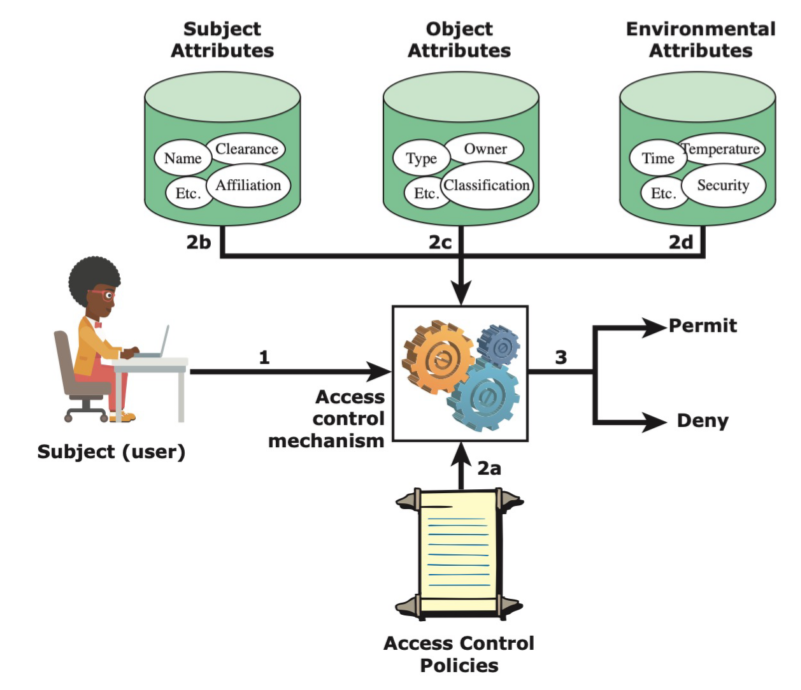
\includegraphics[width=.4\linewidth]{04-access_control/abac}
    \vspace{-8pt}
\end{center}

\begin{enumerate}
    \item A subject requests access to an object. This request is routed to an access control mechanism.
    \item The access control mechanism is governed by a set of rules (2a) that are defined by a preconfigured access control policy. Based on these rules, the access control mechanism assesses the attributes of the subject (2b), object (2c), and current environmental conditions (2d) to determine authorization.
    \item The access control mechanism grants the subject access to the object if access is authorized and denies access if it is not authorized
\end{enumerate}

\newpage

\paragraph{Architecture Conclusion}
\begin{itemize}
    \item It is clear from the logical architecture that there are independent sources of information used for the access control decision:
    \begin{enumerate}
        \item The system designer can decide which attributes are important for access control with respect to subjects, objects, and environmental conditions.
        \item The system designer or other authority can then define access control policies, in the form of rules, for any desired combination of attributes of subject, object, and environmental conditions.
    \end{enumerate}
    \item It should be evident that this approach is very powerful and flexible.
    \item However, the cost, both in terms of the complexity of the design and implementation and in terms of the performance impact, is likely to exceed that of other access control approaches.
    \begin{itemize}
        \item This is a tradeoff that the system authority must make.
    \end{itemize}
\end{itemize}

\paragraph{ABAC Policies}
\begin{itemize}
    \item A policy is a set of rules and relationships that govern allowable behavior within an organization, based on the privileges of subjects and how resources or objects are to be protected under which environment conditions
    \item Typically, it is written from the perspective of the object that needs protecting and the privileges available to subjects
    \item Privileges represent the authorized behavior of a subject and are defined by an authority and embodied in a policy
    \item Other terms commonly used instead of privileges include rights, authorizations, and entitlements
\end{itemize}

\newpage

\subsubsection{ACL Trust Chain}
\begin{center}
    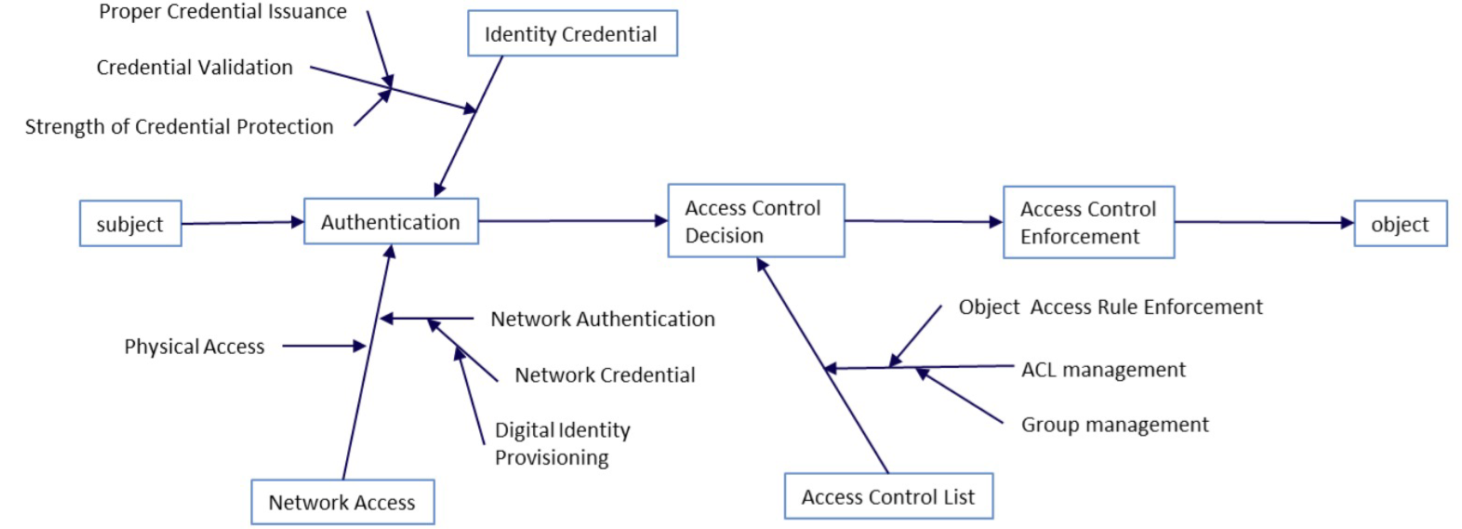
\includegraphics[width=.9\linewidth]{04-access_control/acl_trustchain}
    \vspace{-8pt}
\end{center}

\subsubsection{ABAC Trust Chain}
\begin{center}
    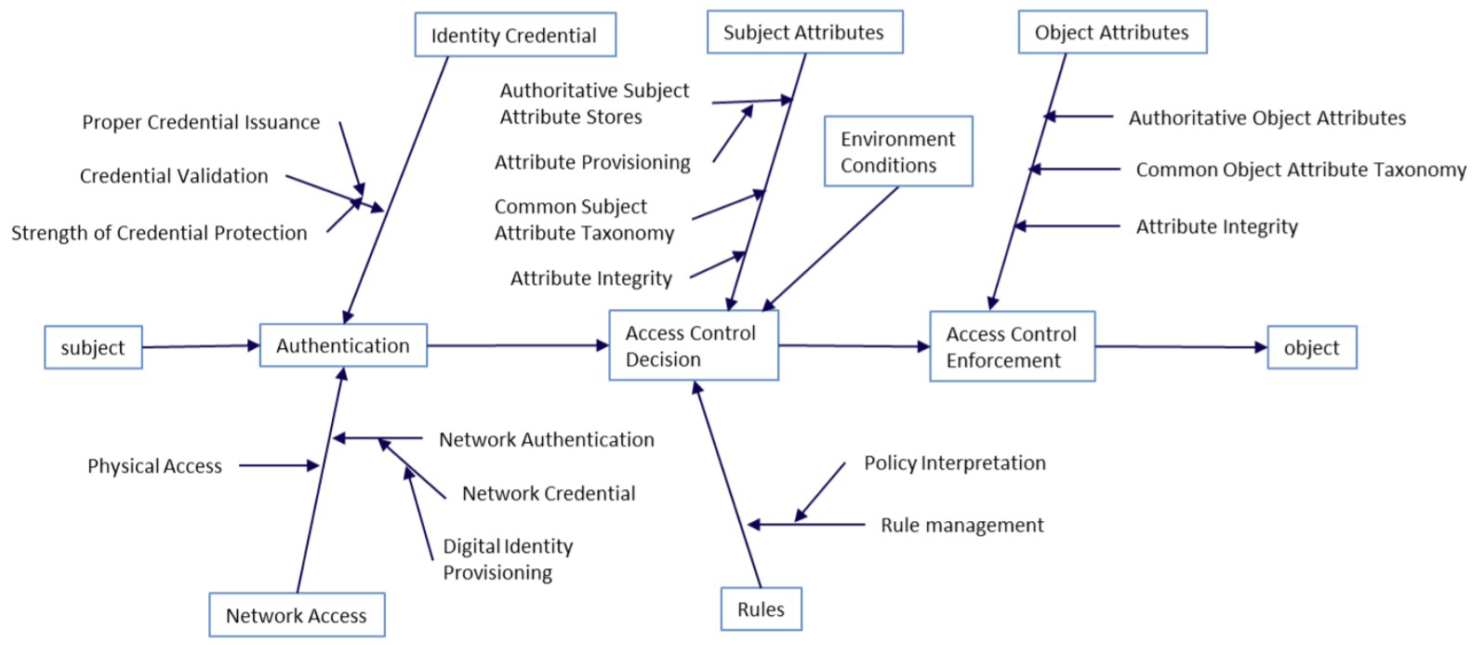
\includegraphics[width=1.0\linewidth]{04-access_control/abac_trustchain}
    \vspace{-8pt}
\end{center}

$subject \rightarrow Authentication \rightarrow Access Control Decision \rightarrow Access Control Enforcement \rightarrow object$\\
ist genau gleich wie bei der ACL Trust Chain $\rightarrow$ Allerdings gibt es zusätzliche Attribute\\

Ein Vergleich von repräsentativen Vertrauensbeziehungen für die Verwendung von ACL und ABAC zeigt, dass es viel komplexere Vertrauensbeziehungen gibt, die erforderlich sind, damit ABAC richtig funktioniert. Ignoriert man die Gemeinsamkeiten in beiden Teilen, kann man feststellen dass bei ACLs die Root of Trust beim ObjectOwner liegt, der letztlich die Objektzugriffsregeln durchsetzt, indem er den Zugriff auf das Objekt durch Hinzufügen eines Benutzers zu einer ACL regelt.

